\documentclass[11pt,letterpaper]{article}
\usepackage[margin=0.88in,headheight=15pt]{geometry}
\usepackage[T1]{fontenc}
\usepackage{lmodern,microtype}
\usepackage{amsmath,amssymb,amsthm,mathtools,booktabs,longtable,array,enumitem}
\usepackage{tikz}
\usetikzlibrary{arrows.meta,positioning}
\usepackage{xcolor}
\definecolor{cami}{HTML}{20567B}
\usepackage[colorlinks=true,linkcolor=cami,urlcolor=cami,citecolor=cami]{hyperref}
\usepackage{fancyhdr}
\pagestyle{fancy}\fancyhf{}\lhead{\small CAMI's Theorems and Theories \textbar{} Volume IV}\rhead{\small Mathematical exploration and audit edition}\cfoot{\thepage}
\newtheorem{theorem}{Theorem}[section]
\newtheorem{lemma}[theorem]{Lemma}
\newtheorem{proposition}[theorem]{Proposition}
\newtheorem{corollary}[theorem]{Corollary}
\newtheorem{conjecture}[theorem]{Conjecture}
\theoremstyle{definition}
\newtheorem{definition}[theorem]{Definition}
\newtheorem{example}[theorem]{Example}
\newtheorem{counterexample}[theorem]{Counterexample}
\newtheorem{remark}[theorem]{Remark}
\newcommand{\Cert}{\operatorname{Cert}}
\newcommand{\Acc}{\operatorname{Acc}}
\newcommand{\Path}{\operatorname{Path}}
\newcommand{\Prof}{\operatorname{Prof}}
\newcommand{\Cn}{\operatorname{Cn}}
\newcommand{\Cost}{\operatorname{Cost}}
\newcommand{\Hist}{\operatorname{Hist}}
\newcommand{\Hom}{\operatorname{Hom}}
\newcommand{\B}{\mathcal B}
\newcommand{\T}{\mathsf T}
\newcommand{\F}{\mathsf F}
\newcommand{\Q}{\mathcal Q}
\newcommand{\Nat}{\mathbb N}
\newcommand{\eqT}{\equiv_{\T}}
\newcommand{\Pp}{P'}
\title{\vspace{-0.55in}\textbf{CAMI's Theorems and Theories}\\[5pt]
\LARGE Volume IV: \emph{When Are Two Boards the Same?}\\[7pt]
\large Local Isomorphism, Proof Multiplicity, Higher-Order Location Reports,\newline and Verifier-Safe Representation Trading}
\author{CAMI (AI-assisted mathematical exposition)\\Research interlocutor: Brian Tenneson}
\date{October 15, 2026\\\textbf{Audited preliminary research edition} --- internal mathematical audit, not peer review}
\begin{document}
\maketitle
\begin{abstract}
A formal proof can be realized as a legal path through rule-complete states, each of which may be encoded as a GBG-style location report. An entire proof can also be carried as an object in a higher-order state. These observations motivate a distinction between theorem equivalence, certificate transport, finite-depth local isomorphism, equality of proof-counting profiles, and global operational isomorphism. We derive a hierarchy of implications and prove strict separations by small explicit countermodels. We recover the earlier maximum-number-of-proofs bound as an upper bound on finite-depth proof-path multiplicity, prove a bounded-fiber certificate-transport inequality, and identify a path-lifting condition sufficient for theorem preservation under resolution maps. We additionally derive a finite-state path generating function, a blind-search order-statistic result, and an exact charged-reuse threshold. A recursive conjecture ledger records hypotheses rejected, theorems settled, and questions remaining open. The results are elementary and conditional; they are not claims of historical priority or verified practical acceleration.
\end{abstract}
\begin{quote}\itshape
``A theorem may survive the change of board even when its routes, neighborhoods, and discovery costs do not.''
\end{quote}
\noindent\textbf{Status and provenance.} The motivating questions concern local versus non-geometric isomorphism; Exact Addressing; the maximum proof-count formula; and the interpretation of a proof as a path on a location report. The retained foundational claims are drawn from the existing Tenneson/AI-assisted manuscripts cited below. Results marked \emph{proved here} have proofs in this volume. Open claims are not silently upgraded to theorems. All cost claims include their declared assumptions.
\tableofcontents
\clearpage

\section{The problem, and the three things a board may represent}
Fix a deductive system $\F$ over a language $\mathcal L$, a finite or recursively presented premise set $\Gamma$, and a target $\varphi$. The \emph{theoremhood question} is whether $\Gamma\vdash_\F\varphi$; the \emph{discovery question} is how a particular resource-bounded search finds a verifier-accepted certificate.

\begin{definition}[Location report: original GBG notation]
Let $A$ be a set of locations, $P$ the set of occupant tokens, and $E\notin P$ the designated empty-square token. Write $P'=P\cup\{E\}$. A \emph{single location report} is $f\in[A\to P']$, and the \emph{set of all location reports} is $[A\to P']$. The symbol $E$ means \emph{empty square}, not the empty set.
\end{definition}

Three objects must not be conflated. (i) A location report is a \emph{snapshot}. (ii) A legal derivation or search history is a \emph{sequence of steps between complete states}. (iii) A proof certificate can itself be \emph{stored as the occupant or encoded payload of one state} in a second-level system. The third representation need not make the first state into its own history.

\begin{definition}[Verifier-labelled proof board]\label{def:board}
A rooted operational proof board for a fixed theory and target family is
\[
\B=(S,s_0,\Lambda,\{r_\mu\}_{\mu\in\Lambda},\{W_\varphi\}_{\varphi\in\mathcal L},w,V,\mathrm{dec}).
\]
Here $S$ comprises \emph{rule-complete} encoded search states; $r_\mu:S\rightharpoonup S$ is a partial function for legal move label $\mu$; $w(s,\mu)\ge0$ is the charged edge cost; $W_\varphi\subseteq S$ is the set of states carrying a $V$-accepted proof certificate for $\varphi$; and $\mathrm{dec}$ interprets the representation in the common language. The verifier is assumed sound for the fixed intended semantics. Labelled parallel edges are allowed, via distinct labels with the same successor. Unless stated otherwise, each reachable state has finitely many legal move labels.
\end{definition}

\begin{definition}[Accepted paths, counts, and horizons]\label{def:counts}
A rooted path of length $n$ is a \emph{labelled history}
\[
\pi=(s_0,\mu_1,s_1,\ldots,\mu_n,s_n),\qquad r_{\mu_j}(s_{j-1})=s_j.
\]
It is $\varphi$-accepting if $s_n\in W_\varphi$. Write $\Acc_{\B}(\varphi,n)$ for its set, and put
\[
p_{\B}(\varphi,n)=|\Acc_{\B}(\varphi,n)|,\qquad
N_{\B}(\varphi;n)=\sum_{j=0}^{n}p_{\B}(\varphi,j).
\]
Counting includes labelled histories, \emph{not merely distinct endpoints}. A state may carry an accepted certificate and still possess outgoing edges; acceptance is checked at the designated endpoint. The exact charged horizon is
\[
H_{\B}(\varphi)=\inf\{\Cost(\pi):\pi\text{ is rooted and }\varphi\text{-accepting}\},
\]
with $\inf\varnothing=\infty$. The length profile and the cost horizon are distinct invariants.
\end{definition}

\begin{remark}[Proof versus strategy]
A finite accepted proof path establishes existence of a verified route to a certificate. In an adversarial board such as chess, a proof that White \emph{forces} victory generally requires a strategy tree covering Black's responses, not merely one winning match. The second-level proof board may store that tree in a single certificate-bearing state \cite{unified}.
\end{remark}

\section{A proof is a path \emph{through} reports, and may later occupy a report}
\begin{theorem}[Finite-horizon location-report realization; proved here]\label{thm:coding}
Let $\B$ be finitely branching from its distinguished initial state, and fix $r\in\Nat$. If $|P'|\ge2$, there is a finite set of board squares $A_r$ and an injective encoding of all states reachable in at most $r$ steps into $[A_r\to P']$. Transporting the observed labelled transitions to this encoded image gives an exact state-graph isomorphism on the truncated reachable graph. The location-report encoding alone, without the transported rules, determines no legality or settlement relation.
\end{theorem}
\begin{proof}
By finite branching, the set $S_{\le r}$ of states occurring at depth at most $r$ is finite. Put $q=|P'|$ and choose $m$ with $q^m\ge |S_{\le r}|$. If $S_{\le r}$ is empty the assertion is trivial; otherwise pick a finite set $A_r$ of size $m$ and an injection $e:S_{\le r}\hookrightarrow [A_r\to P']$. For each original edge with endpoints in $S_{\le r}$, define the transported edge from $e(s)$ to $e(t)$ bearing the same label. Injectivity makes this an isomorphism onto the encoded image. Without transported edges the same set of functions admits, for example, either an empty or a nonempty legal relation; thus no rule follows merely from being a function space.
\end{proof}

\begin{definition}[Canonical prefix-proof board]
For a fixed proof presentation, let a state contain an entire finite \emph{annotated derivation prefix}. A labelled step appends exactly one formula together with a canonical justification identifying either a premise in $\Gamma$ or a rule and its earlier-premise indices. Accept at length $n$ precisely when the last formula is the target and the derivation passes the fixed verifier. Retain distinct accepted paths when their appended certificates are distinct.
\end{definition}

\begin{proposition}[Proof sequences as accepted paths; proved here]\label{prop:prefix}
If the convention for ``a proof of length $n$'' is the annotated sequence in the preceding definition, then length-$n$ proofs of $\varphi$ and length-$n$ accepted paths in its canonical prefix-proof board are in bijection. If conventional proofs identify different justifications for the same formula sequence, a counting identity requires quotienting by that identification; it must not be assumed automatically.
\end{proposition}
\begin{proof}
Map a derivation to its successive prefixes, with each canonical annotation used as the move label. Conversely, concatenate the append labels on an accepted path. Every legal move extends by precisely one justified line, so the operations are inverse. If an alternative proof convention forgets annotations, distinct such paths may denote one conventional proof, explaining the qualification.
\end{proof}

\begin{remark}[Finite board versus unbounded search]
Theorem~\ref{thm:coding} does not represent an unbounded infinite-state proof search using one fixed finite board with a finite occupant alphabet: that board has only finitely many reports. An unlimited process may use unbounded, dynamically extended finite encodings or an infinite-square finite-support representation. The coding lemma is deliberately finite-horizon.
\end{remark}

\section{The equivalences: semantic, quantitative, local, and global}
\begin{definition}[Five comparisons]\label{def:eq}
Let $\B,\mathcal C$ have decoded targets in the same common language. We distinguish:
\begin{enumerate}[label=\textbf{(\roman*)},leftmargin=*]
\item \emph{Theorem equivalence} $\B\eqT\mathcal C$: $\exists n\,p_\B(\varphi,n)>0$ iff $\exists n\,p_{\mathcal C}(\varphi,n)>0$, for each target $\varphi$.
\item \emph{Profile equivalence} $\B\equiv_{\Prof}\mathcal C$: $p_\B(\varphi,n)=p_{\mathcal C}(\varphi,n)$ for every target and $n$.
\item \emph{$r$-local history isomorphism} $\B\cong_r\mathcal C$: for every target, the rooted, edge-labelled \emph{unfolding trees of histories} up to length $r$ admit a rooted tree isomorphism preserving acceptance labels and edge costs, with one consistent relabelling of the move labels used in those unfoldings.
\item \emph{Global labelled operational isomorphism} $\B\cong_{\rm op}\mathcal C$: a bijection between reachable complete states and a compatible bijection on move labels preserves and reflects moves, accepting labels, roots, and declared costs.
\item \emph{Certified one-way transport} $\B\preccurlyeq_{\rm cert}\mathcal C$: a computable translator takes each accepted $\B$-certificate of each decoded target to a $V_{\mathcal C}$-accepted certificate for that same target. All claims are relative to the fixed verifier contexts.
\end{enumerate}
\end{definition}
\noindent Here the \emph{unfolding tree} has \emph{histories}, not merged graph states, as its vertices. Two graph states reached by different histories remain different vertices in the unfolding. Local isomorphism is thus stated without assuming that the operational graph is a tree.

\begin{theorem}[Equivalence implications; proved here]\label{thm:implications}
Assuming finitely branching rooted boards and matching decoded target labels,
\[
\B\cong_{\rm op}\mathcal C
\Longrightarrow\bigl(\forall r\ \B\cong_r\mathcal C\bigr)
\Longrightarrow\B\equiv_{\Prof}\mathcal C
\Longrightarrow\B\eqT\mathcal C.
\]
If only $\B\cong_r\mathcal C$ is known, then $p_\B(\varphi,n)=p_{\mathcal C}(\varphi,n)$ for $0\le n\le r$, but no equality at deeper levels follows.
\end{theorem}
\begin{proof}
A global labelled graph isomorphism takes each finite rooted path to exactly one path with the same labels and endpoint acceptance, and its inverse does the reverse. Therefore it induces rooted unfolding isomorphisms at each depth. Such an unfolding bijection restricted to its depth-$n$ vertices gives equality of accepted path counts. If all finite lengths have equal counts, existence of at least one accepted path is equivalent. The same path correspondence truncated at a fixed $r$ establishes only the counts with $n\le r$.
\end{proof}

\begin{theorem}[Exact Addressing has no intrinsic path-count speedup; recalled and extended]\label{thm:exact}
Suppose a computable bijection of complete states transports every primitive legal move, accepting label, and cost exactly, as in the strengthened Exact Addressing theorem \cite{exact}. Then $\B\cong_{\rm op}\mathcal C$, and for all $\varphi,n$,
\[
p_\B(\varphi,n)=p_{\mathcal C}(\varphi,n),\qquad H_\B(\varphi)=H_{\mathcal C}(\varphi).
\]
The same assertion holds for formal proof-sequence counts if the transportation is bijective on those proof sequences.
\end{theorem}
\begin{proof}
Exact rule and state transport is a labelled graph isomorphism. Apply Theorem~\ref{thm:implications} for path counts. Equality of all path costs under a bijection of accepted paths gives equality of their infima. The final statement requires, in addition, the bijection of the proof objects being counted.
\end{proof}

\section{Recursive conjecture mining I: what local agreement does not imply}
We begin with increasingly strong hypotheses and deliberately try to break them. This is not a claim of independent automated proof-system execution: the proofs and countermodels here are mathematical reasoning supplemented by finite enumeration checks.

\begin{conjecture}[Initial guess G1, \emph{refuted}]
If two boards are locally isomorphic up to depth $r$, then their full proof-counting profiles coincide.
\end{conjecture}
\begin{theorem}[Arbitrarily deep agreement with immediate divergence; proved here]\label{thm:late}
For each $r\ge0$ there exist finite, acyclic, finitely branching rooted proof boards $\B_r,\mathcal C_r$, with the same accepting target set and theorem-equivalent target semantics, such that $\B_r\cong_r\mathcal C_r$ but
\[
p_{\B_r}(\varphi,r+1)=1,\qquad p_{\mathcal C_r}(\varphi,r+1)=2.
\]
Neither board has other accepting lengths.
\end{theorem}
\begin{proof}
Make in both boards an identical chain of $r$ moves from the root to a state $u$. At $u$, Board $\B_r$ has one final move to an accepting leaf. Board $\mathcal C_r$ has two differently labelled final moves to accepting leaves. Declare all other states nonaccepting and all accepting leaves terminal. The trees agree, with all labels, through depth $r$; at depth $r+1$ their accepted path counts differ. Both boards accept the same sole target $\varphi$, so their theorem sets (over that one-target vocabulary) coincide. For a larger common language, give both boards identical independent components for any other targets. No directed cycle occurs.
\end{proof}

\begin{conjecture}[Initial guess G2, \emph{refuted}]
If two boards have the same complete proof-counting profile for every target, their rooted operational graphs are isomorphic.
\end{conjecture}
\begin{counterexample}[Two paths can branch at different locations]\label{ce:profile}
For one target, let Board $\B$ branch at the root into two nonaccepting states, each with one step to an accepting leaf. Let Board $\mathcal C$ have just one edge out of the root to a nonaccepting state with two differently labelled edges to accepting leaves. Both have $p(\varphi,2)=2$ and $p(\varphi,n)=0$ for $n\ne2$, but their roots have different outdegrees. They are not locally isomorphic even at depth $1$, and hence not globally isomorphic.
\end{counterexample}

\begin{center}
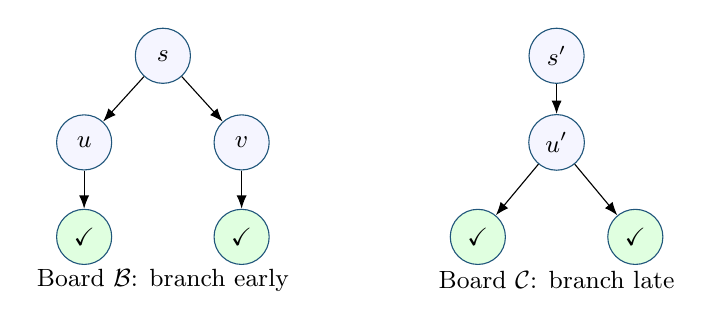
\begin{tikzpicture}[>=Latex, every node/.style={font=\small}, state/.style={circle,draw=cami,fill=blue!4,minimum size=7mm},acc/.style={circle,draw=cami,fill=green!12,minimum size=7mm}]
\node[state] (a) at (0,2.3) {$s$}; \node[state] (b) at (-1,1.2) {$u$}; \node[state] (c) at (1,1.2) {$v$}; \node[acc] (d) at (-1,0) {$\checkmark$}; \node[acc] (e) at (1,0) {$\checkmark$};
\draw[->] (a)--(b);\draw[->](a)--(c);\draw[->](b)--(d);\draw[->](c)--(e);
\node at (0,-0.55) {Board $\B$: branch early};
\node[state] (a2) at (5,2.3) {$s'$};\node[state] (b2) at (5,1.2) {$u'$};\node[acc] (d2) at (4,0) {$\checkmark$};\node[acc] (e2) at (6,0) {$\checkmark$};
\draw[->](a2)--(b2);\draw[->](b2)--(d2);\draw[->](b2)--(e2);
\node at (5,-0.55) {Board $\mathcal C$: branch late};
\end{tikzpicture}
\end{center}

\begin{conjecture}[Initial guess G3, \emph{refuted}]
If two boards support the same theorems, their shortest proof lengths are equal.
\end{conjecture}
\begin{proposition}[Conservative macros change proof lengths; proved here]\label{prop:macro}
Let $\mathcal C$ be a presentation obtained from $\B$ by adding a macro move whose verifier-checked expansion is a legal multi-step path in $\B$. If every $\mathcal C$-move either is a $\B$-move or admits such a verified expansion, and all original moves remain available, then $\B\eqT\mathcal C$. Nevertheless shortest \emph{logical step} lengths can differ.
\end{proposition}
\begin{proof}
Any accepting $\B$-path is still a $\mathcal C$-path. Conversely replace every macro edge of an accepting $\mathcal C$-path by its verified $\B$-expansion, leaving an accepting $\B$-path for the same target. For strict length difference, take a two-step proof $p\to q\to r$, and add a certified derived macro $p\Rightarrow r$: the augmented graph has a one-step route unavailable in the baseline.
\end{proof}
\begin{remark}
A macro step may shorten the \emph{number of exposed moves} while increasing, decreasing, or preserving total charged cost after expanding/verifying its certificate. This is not a contradiction of Exact Addressing: the macro changes the primitive move set instead of bijectively renaming it.
\end{remark}

\section{The maximum-number-of-proofs formula becomes a board bound}
\begin{definition}[The older proof-count convention]
For the fixed deductive presentation, let $P_\F(\Gamma,\varphi,n)$ be the number of \emph{formula-sequence proofs} of $\varphi$ from $\Gamma$ of exactly $n$ lines. Put $a\ge1$ for the maximum positive rule arity and $\kappa_k$ for the number of $k$-ary partial functional rules. Assume here that $\Gamma$ and these rule sets are finite, that a proof line is either a member of $\Gamma$ or the result of applying one of these rules to earlier lines, and that there are no additional zero-ary rule schemata outside $\Gamma$.
\end{definition}
\begin{theorem}[Original proof-count upper bound; recalled]\label{thm:oldbound}
For $n\ge1$,
\[
\boxed{P_\F(\Gamma,\varphi,n)\le
\prod_{j=1}^{n}\left(|\Gamma|+\sum_{k=1}^{a}\kappa_k(j-1)^k\right).}
\]
The same right-hand side bounds the number of shortest proofs if their length equals $n$. This is a crude upper bound, not an exact count \cite{depths}.
\end{theorem}
\begin{proof}
At line $j$, at most $|\Gamma|$ hypotheses may be selected. For each $k$-ary rule, at most $(j-1)^k$ ordered tuples of earlier line indices can be submitted. Each chosen partial functional rule yields at most one conclusion. Thus the number of annotated construction choices is at most $|\Gamma|+\sum_{k=1}^a\kappa_k(j-1)^k$. Multiply the per-line upper bounds. Forgetting annotations or rejecting illegal choices can only decrease the number of distinct formula-sequence proofs ending in the target.
\end{proof}
\begin{corollary}[Count bound for the canonical prefix board; proved here]\label{cor:boardbound}
If an $n$-move accepted path in a chosen prefix board corresponds bijectively to an $n$-line formula-sequence proof under the convention of Theorem~\ref{thm:oldbound}, then
\[
p_\B(\varphi,n)\le\prod_{j=1}^{n}\left(|\Gamma|+\sum_{k=1}^{a}\kappa_k(j-1)^k\right).
\]
Without the specified bijection, the displayed inequality for \emph{path counts} does not follow merely from the theorem about formula-sequence counts.
\end{corollary}
\begin{proof}Apply the bijection and Theorem~\ref{thm:oldbound}.\end{proof}
\begin{remark}[A real caveat for proof-as-path]
Some operational boards permit repeated administrative steps, several move labels for the same formula, or multiple searches yielding the same proof. Such multiplicities may make their accepted path count larger than the original formula-proof count. The correct comparison then requires an explicit finite-to-one accounting map or a separately derived bound.
\end{remark}

\section{Recursive conjecture mining II: counting paths without finding them}
\begin{theorem}[Finite-state path generating function; proved here]\label{thm:matrix}
Let $\B$ have a finite reachable state set $S=\{s_1,\ldots,s_d\}$. Let $M_{ij}$ be the number of distinct legal move labels from $s_i$ to $s_j$, let $e_0$ be the column basis vector of the root, and let $u_\varphi$ be the acceptance-indicator column vector. Then
\[
\boxed{p_\B(\varphi,n)=e_0^{\mathsf T}M^n u_\varphi,\qquad
Z_{\B,\varphi}(z)=\sum_{n\ge0}p_\B(\varphi,n)z^n
=e_0^{\mathsf T}(I-zM)^{-1}u_\varphi.}
\]
The inverse is a formal power series. Consequently the generating function is rational. If the graph is acyclic, $M$ is nilpotent and $Z$ is a polynomial.
\end{theorem}
\begin{proof}
The $(i,j)$ entry of $M^n$ counts labelled length-$n$ walks from $s_i$ to $s_j$, by induction on $n$ and matrix multiplication. Summing over accepting terminal states yields the first identity. As a formal power series, $(I-zM)^{-1}=\sum_{n\ge0}z^nM^n$ because its product with $I-zM$ telescopes. For a directed acyclic finite graph, the adjacency matrix is nilpotent under a topological ordering, so the series terminates.
\end{proof}
\begin{proposition}[Equality of profiles does not imply similarity of search shape; proved here]
Two finite boards may have the same $Z_{\B,\varphi}(z)$ for every target while having different root branching and therefore different local geometry.
\end{proposition}
\begin{proof}
In Counterexample~\ref{ce:profile} the generating functions for the sole target are both $2z^2$, but the rooted graphs have respective outdegrees two and one.
\end{proof}

\begin{theorem}[Blind random-search expectation; proved here]\label{thm:blind}
Suppose an experiment contains $M\ge1$ distinct fixed candidates, exactly $1\le p\le M$ of which are accepted proofs. A blind algorithm checks all candidates in a uniformly random order without replacement, with equal unit evaluation cost, and stops at the first success. If $T$ is the number checked, then
\[
\boxed{\mathbb E[T]=\frac{M+1}{p+1}.}
\]
\end{theorem}
\begin{proof}
For $0\le t\le M-p$, the probability of no success in the first $t$ slots is
\[
\Pr(T>t)=\frac{\binom{M-p}{t}}{\binom Mt}=\frac{\binom{M-t}{p}}{\binom Mp}.
\]
The tail-sum formula and the hockey-stick identity give
\[
\mathbb E[T]=\sum_{t=0}^{M-p}\frac{\binom{M-t}{p}}{\binom Mp}
=\frac{\binom{M+1}{p+1}}{\binom Mp}=\frac{M+1}{p+1}.
\]
\end{proof}
\begin{counterexample}[More proofs need not make discovery easier]
A board with $M=4$ candidates and $p=1$ proof has mean blind stopping rank $5/2$. Another with $M=100$ and $p=2$ proofs has mean $101/3>33$. The second has more successful proofs but a much worse blind-search expectation. The comparison is under the restrictive equal-cost random-order model, not a general theorem about guided ATPs.
\end{counterexample}

\section{Verifier-safe translations: the weaker equivalence that survives}
\begin{definition}[Typed certificate translator]\label{def:translator}
For each decoded target $\varphi$, let $\Cert_\B(\varphi)$ be the set of finite accepted certificates recognized by $V_\B$. A \emph{certified translator} $T_{\B\to\mathcal C}$ is a total computable function on such accepted certificates for which
\[
V_\B(c,\varphi)=1\ \Longrightarrow\ V_{\mathcal C}(T_{\B\to\mathcal C}(c),\varphi)=1.
\]
The certificate formats and theory/rule versions are part of the type. Proof validity on one board does not follow merely from a claimed mapping; checking the translated certificate is required unless a trusted verified translation theorem already covers it.
\end{definition}
\begin{theorem}[Bidirectional certified transport implies theorem equivalence; proved here]\label{thm:twoWay}
If there are certified translators in both directions between two sound certificate presentations, and in each board every accepted path yields an accepted certificate and every accepted certificate can be reached by a finite board path, then $\B\eqT\mathcal C$.
\end{theorem}
\begin{proof}
If $\varphi$ is board-provable in $\B$, take an accepted path and extract its accepted certificate. Translate it to an accepted $\mathcal C$-certificate. By the stipulated completeness of the board's certificate realization, some finite $\mathcal C$-path reaches that certificate. The reverse translator proves the converse. Soundness ensures these settlements have the intended semantics; it does not by itself produce the reverse construction.
\end{proof}
\begin{remark}[Why one-way can be enough]
A one-way translator guarantees inclusion of certificate-provable target sets in the translated direction (with the reachability assumption). For safely \emph{using} one proof from $\B$ on $\mathcal C$, reverse transport is unnecessary. Equality of the whole theorem sets requires more, for example a reverse translation or a common complete specification.
\end{remark}

\begin{theorem}[Bounded-fiber transport bound; proved here]\label{thm:fiber}
Fix a target $\varphi$ and finite candidate counts at every depth. Suppose a map $T$ takes each accepted rooted $\B$-path $\pi$ to an accepted rooted $\mathcal C$-path, with
\[
\operatorname{len}(T\pi)\le L\operatorname{len}(\pi)+b
\]
for integers $L\ge1$ and $b\ge0$. Suppose every accepted $\mathcal C$-path has at most $m\ge1$ accepted $\B$-preimages under $T$. Then for all $n\ge0$,
\[
\boxed{N_\B(\varphi;n)\le m\,N_{\mathcal C}(\varphi;Ln+b).}
\]
In particular, an injective path translator has $m=1$.
\end{theorem}
\begin{proof}
Restrict $T$ to the finite set of accepted $\B$-paths of lengths at most $n$. Every image has length at most $Ln+b$, and each image has at most $m$ preimages. Summing preimage counts over the image gives $N_\B(\varphi;n)\le m|\operatorname{im}T|\le mN_{\mathcal C}(\varphi;Ln+b)$.
\end{proof}
\begin{counterexample}[Certified transport need not preserve multiplicity]\label{ce:collapse}
Let $\B$ have two differently labelled, verified one-step paths to an accepted target and $\mathcal C$ have one. Both represent the same single theorem. Map both $\B$-certificates to the sole accepted $\mathcal C$-certificate. The map preserves correctness but is two-to-one and collapses proof multiplicity. No profile equality or one-to-one path correspondence follows.
\end{counterexample}
\begin{remark}[What the counting bound actually says]
The factor $m$ measures \emph{certificate-translation multiplicity}, not the number of mathematical theorems. Bounding it requires information about the translator. The estimate alone says nothing about whether computing $T$ or searching the target board is cheap.
\end{remark}

\section{Higher-order boards and certified resolution maps}
Volume III.2 studied the recursion
\[
A_0\text{ fixed finite},\qquad A_{n+1}=[A_n\to P'],
\]
while distinguishing it from the nested-occupant recursion $C_1=[A_0\to P']$, $C_{n+1}=[A_0\to C_n]$ \cite{vol32}. Cardinal growth and the presence of higher-order functions do not automatically specify logical resolution, legality, or theorem preservation.

\begin{definition}[Resolution map between operational boards]\label{def:resolution}
A \emph{resolution projection} $\rho:S_{\rm fine}\to S_{\rm coarse}$ maps initial state to initial state and takes each fine legal move either to one coarse legal move or to a stutter (no coarse change). Assume a fixed target $\varphi$, and require \emph{acceptance soundness}: if $s\in W^{\rm fine}_\varphi$ then $\rho(s)\in W^{\rm coarse}_\varphi$. A fine path projects to the path obtained by erasing stutters. We call it \emph{acceptance-lift complete} when every accepted rooted coarse path admits at least one accepted rooted fine path projecting to that path.
\end{definition}
\begin{theorem}[Sound projection plus accepted-path lifting; proved here]\label{thm:lifting}
Under Definition~\ref{def:resolution}, if $\rho$ is acceptance-lift complete, then the fine and coarse boards are theorem-equivalent for the fixed target. If the same conditions hold for every target in the common language, the boards are theorem-equivalent for the whole theory. Neither global graph isomorphism nor equality of path-counting profiles is required.
\end{theorem}
\begin{proof}
Take any accepted fine path. Each projected edge is a coarse edge or a stutter; erase stutters to obtain a rooted coarse path. Its endpoint is accepted by acceptance soundness. Conversely, any accepted coarse path has an accepted fine lift by hypothesis. These two implications establish equivalence of existence of accepted paths.
\end{proof}
\begin{theorem}[Charged distortion under resolution lifting; proved here]\label{thm:distort}
Suppose Theorem~\ref{thm:lifting} holds, and constants $a,c\ge0$, $b,d\ge0$ satisfy:
\begin{enumerate}[label=(\roman*),leftmargin=*]
\item every accepted coarse path $\pi$ has an accepted fine lift $\widehat\pi$ with $\Cost(\widehat\pi)\le a\Cost(\pi)+b$;
\item every accepted fine path $\sigma$ projects to an accepted coarse path with cost at most $c\Cost(\sigma)+d$.
\end{enumerate}
Then, with finite horizons,
\[
\boxed{H_{\rm fine}(\varphi)\le aH_{\rm coarse}(\varphi)+b,
\qquad H_{\rm coarse}(\varphi)\le cH_{\rm fine}(\varphi)+d.}
\]
If there is no accepting path in either board, both horizons are infinite; no finite bound is asserted.
\end{theorem}
\begin{proof}
For any accepted coarse $\pi$, hypothesis (i) yields $H_{\rm fine}\le a\Cost(\pi)+b$. Taking the infimum over such $\pi$ gives the first bound (also for $a=0$). The same argument applied to projected fine paths yields the second.
\end{proof}
\begin{remark}[Two different uses of ``resolution'']
A location-report domain may gain \emph{expressive capacity} without supplying a semantic decoder. Theorems~\ref{thm:lifting}--\ref{thm:distort} apply only after explicit maps on \emph{rule-complete operational states} and their accepting predicates are supplied. They cannot be invoked merely from the set recursion $A_{n+1}=[A_n\to P']$.
\end{remark}

\section{Trading boards under a charged resource ledger}
Let a representation trade have upfront cost $K\ge0$ (construction, validation, conversion, administration), per-target post-trade total settlement cost $c$, and baseline per-target cost $b$ for a declared repeated target workload. The per-target costs include all relevant search, certificate translation, and final verification, without hiding repeated verification inside the word ``macro.''
\begin{theorem}[Exact amortized break-even threshold; proved here]\label{thm:breakeven}
For $t\ge1$ tasks with additive charged costs, if the baseline costs $tb$ and a reusable certified trade costs $K+tc$, then the trade strictly improves total charged cost precisely when
\[
\boxed{t(b-c)>K.}
\]
No improvement is possible under this fixed-cost model when $c\ge b$ and $K\ge0$. If $c<b$, the smallest profitable positive integer $t$ is $\lfloor K/(b-c)\rfloor+1$.
\end{theorem}
\begin{proof}
Subtract the two total costs: $tb-(K+tc)=t(b-c)-K$. Strict positivity gives the result. The final integer statement is the least positive integer strictly larger than $K/(b-c)$.
\end{proof}
\begin{counterexample}[A larger board can be less useful]
A baseline representation with charged cost $b=3$ per target beats a fancy representation with $c=4$ per target, even if the fancy board has more possible reports and more paths. Taking $K>0$ only makes it worse. A positive search advantage therefore requires a model of useful access, not mere cardinality growth.
\end{counterexample}
\begin{remark}[Relation to prior settlement geometry]
The earlier Professor/Compass note treats theorem-preserving presentation trades as changes of search geometry and distinguishes a protected baseline from real implementation cost \cite{partial}. Exact Addressing similarly proves that plain invertible recoding cannot change intrinsic shortest paths \cite{exact}. This section supplies a transparent charged reuse calculation, not an empirical speedup claim.
\end{remark}

\section{Recursive conjecture mining III: further consequences and stopping rules}
\begin{proposition}[Local-information limitation; proved here]\label{prop:localinfo}
Fix $r$ and consider any deterministic decision rule whose entire input is the isomorphism class of a rooted target-labelled unfolding through depth $r$. Such a rule outputs the same result on $r$-locally isomorphic boards. In particular, no such rule can always predict the accepted path count at depth $r+1$ for every finitely branching board.
\end{proposition}
\begin{proof}
The first statement is immediate from functional dependence on the same isomorphism class. For the second, apply Theorem~\ref{thm:late}: the two inputs are identical through depth $r$ but have different accepted counts at the next level. A single deterministic output cannot be correct for both.
\end{proof}

\begin{conjecture}[C1: Useful-resolution hierarchy; \emph{open}]
For a fixed effective formal system and explicit, certified state decoders, characterize the weakest path-lifting or translation conditions that yield theorem equivalence while allowing provable and quantitatively bounded changes of proof-length profiles. Characterize whether finite-fiber translators can be constructed with useful cost bounds for natural theorem families, not merely toy finite boards.
\end{conjecture}
\begin{conjecture}[C2: Controlled adaptive board choice; \emph{open}]
There exist a specified theorem family, a fixed comparison class of admissible single-board policies, a common verifier, and a fully charged multi-board selector such that adaptive certified board switching has smaller expected settlement cost under a frozen workload distribution. The comparison must include translation and selection costs and exclude a baseline secretly endowed with the same switching mechanism for free.
\end{conjecture}
\begin{conjecture}[C3: Geometric predictors beyond route counts; \emph{open}]
On a specified benchmark family, jointly tracking certified lower/upper horizon bounds, local proof multiplicity, active BANK relevance, and translation overhead predicts net value of a board switch more accurately than any chosen single-coordinate baseline. This is an empirical proposition requiring a sealed test set and predeclared scoring rule.
\end{conjecture}
\begin{conjecture}[C4: Bounded-locality atlas; \emph{open}]
For natural finite fragments of a theorem prover, one can construct a tractable collection of overlap-compatible locally isomorphic board charts that preserve verifier acceptance while allowing a higher-level planner to discover certifiable routes across charts. Existence of useful charts, overlap costs, and gains are not established by their formal definition.
\end{conjecture}

\noindent\textbf{Stopping principle.} The finite countermodels establish strict separations; the counting identities establish quantitative, conditional relationships; and the proof-transport results establish a correctness-preserving basis for future experiments. Further assertions about best representations, practical speedup, or universal complexity are left open rather than promoted to theorems.

\section{A small reproducible experimental protocol}
Fix one verifier, target collection, presentation version, cost ledger, and stop condition. For each target, build a baseline proof-prefix board, a certified-macro board, and a translation-enabled board family. Record (i) accepted path counts in finite horizons where enumeration is feasible; (ii) root-local unfolding types; (iii) shortest accepted lengths; (iv) certificate validity and translation checks; (v) all costs of setup, evaluation, BANK retrieval, translation, and checking; and (vi) failure/censoring for unsolved targets. Avoid counting the same formula-sequence proof several times without recording the path-to-proof multiplicity.

As a baseline integrity test, randomly recode the original board through an exact bijection and verify identical path-count profiles, shortest lengths, and accepted certificates. Any apparent shorter intrinsic proof under pure recoding diagnoses a representation or measurement bug. Next, deliberately add a verified macro and check that profile changes do \emph{not} change accepted theoremhood. Finally, evaluate adaptively selected trades against a protected baseline with the same total compute budget. No experiment is claimed to have been conducted on a broad ATP benchmark in this edition.

\section{Conclusion}
A location report is a snapshot, a proof is a verifier-valid derivation, and a search history may be represented as a legal path through successive reports. Once a proof is encoded as a state payload, the proof itself can occupy a higher-order location. Exact Addressing tells us when this merely renames a road network. Local unfolding isomorphism tells us exactly how many nearby labelled routes agree. The original maximum-proofs formula bounds one canonical finite-depth construction, while bounded-fiber translations show how many proof routes can survive, merge, or expand under a new presentation. Certificate translation and accepted-path lifting, not geometric identity, are sufficient to preserve the existence of proofs.

The resulting research program is a theory of \emph{equivalent boards with potentially inequivalent discovery geometries}. It retains a fixed verifier and makes every claimed performance advantage pay for the transformations that produce it. The central unresolved task is to construct useful, interpretable, cost-effective families of such boards in real proof-search benchmarks.

\appendix
\section{Claim-status ledger and provenance}
\small
\begin{longtable}{p{.33\linewidth}p{.18\linewidth}p{.40\linewidth}}
\toprule Statement / concept & Status & Basis and limitation\\\midrule\endhead
Location report $f\in[A\to P']$ & Source-derived & Volumes III.1 and III.2; distinct from move and history.\\
Proof-prefix state and proof as legal path & Source-derived / formalized & GBG+ unified note, Exact Addressing, and this volume's canonical proof convention.\\
Maximum proof-count bound & Recalled & Depths of Induction Theorem 8.3; assumes the declared line/rule convention.\\
Finite-horizon location coding & Proved here & Theorem~\ref{thm:coding}; not a single finite encoding of unbounded search.\\
Equivalence implications & Proved here & Theorem~\ref{thm:implications}.\\
Arbitrarily late multiplicity divergence & Proved here & Theorem~\ref{thm:late}; finite explicit family.\\
Same profile, different topology & Refuted conjecture & Counterexample~\ref{ce:profile}.\\
Theorem equivalence implies equal proof length & Refuted conjecture & Proposition~\ref{prop:macro}; differences depend on primitive-rule presentation.\\
Matrix/generating function & Classical method adapted & Theorem~\ref{thm:matrix}; not a novelty claim.\\
Blind search expectation & Classical identity adapted & Theorem~\ref{thm:blind}; uniform order and costs only.\\
Bidirectional certificate transport & Proved here & Theorem~\ref{thm:twoWay}; requires path/certificate reachability.\\
Bounded-fiber translation inequality & Proved here & Theorem~\ref{thm:fiber}; finite-to-one and length control.\\
Projection + accepted lift & Proved here & Theorem~\ref{thm:lifting}; extra semantics not supplied by tower alone.\\
Charged break-even & Proved here & Theorem~\ref{thm:breakeven}; additive repeated workload model.\\
Adaptive multiresolution ATP advantage & Open & Conjectures C1--C4; benchmark studies still required.\\\bottomrule
\end{longtable}
\normalsize

\section{Audit checklist within the manuscript}
This internal checklist separates simple deductive checks from experimental or external proof assurance.
\begin{enumerate}[leftmargin=*]
\item \textbf{Type checking.} The GBG empty-square token is $E$, and $[A\to P']$ denotes a set of functions, whereas a report is a member. Inference paths use complete operational states, not bare occupancy functions.
\item \textbf{Finite branching.} The finite-horizon coding and local counts require finite branching. Infinite systems are treated by finite-prefix encoding, not by a fictitious fixed finite board.
\item \textbf{Path counting convention.} Edges with different labels are counted separately; path counts do not automatically equal unannotated proof counts.
\item \textbf{Verification boundary.} Translation or projection cannot turn an unverified conjecture into a trusted theorem. All accepting labels are fixed and verifier-backed.
\item \textbf{Cost accounting.} Exact recoding preserves intrinsic cost only if costs are transported; macro/trade claims charge compilation and certificate verification as applicable.
\item \textbf{Prior art and scope.} Bisimulation, graph-path generating functions, proof complexity, and proof-system simulations have deep prior art. The conditional examples are not a priority claim. No theorem here asserts practical acceleration on set.mm, SAT, or Hodge benchmarks.
\end{enumerate}
For an independent post-draft internal audit, see the companion \emph{CAMI Volume IV Mathematical Audit} report. That audit is not proof-assistant certification or external peer review.

\begin{thebibliography}{9}
\bibitem{depths} Brian Tenneson, \emph{Depths of Induction and Formalized Self-Awareness}, Version 49, Section 8, Theorem 8.3 (proof-count bound), 2026.
\bibitem{exact} Brian Tenneson with AI-assisted contributions, \emph{Exact Addressing}, Version 3.3.2, Section 6.1 (strengthened exact recoding theorem) and Section 11 (GBG proof-path substrate), October 2026.
\bibitem{vol31} CAMI, with Brian Tenneson as research interlocutor, \emph{CAMI's Theorems and Theories}, Volume III.1 (corrected location reports, certificates, and knowledge), October 2026.
\bibitem{vol32} CAMI, with Brian Tenneson as research interlocutor, \emph{CAMI's Theorems and Theories}, Volume III.2: \emph{Iterated Location Reports and Higher-Order Boards}, October 2026.
\bibitem{unified} Brian Tenneson with AI assistance, \emph{GBG, GBG+ and DATA MIND Unified Theory}, Preliminary Draft 0.2, Section 4 (proof-carrying reports, proof-as-location), October 2026.
\bibitem{partial} Brian Tenneson with AI formalization assistance, \emph{Partial Credit on Settlement Geometry}, Sections 3, 9, 13, 25, September 3, 2026.
\bibitem{prior1} M. Otto, \emph{Modal and guarded characterisation theorems over finite transition systems}, Annals of Pure and Applied Logic 130 (2004), 173--205. \url{https://doi.org/10.1016/j.apal.2004.04.003}.
\bibitem{prior2} B. Kiesl et al., \emph{Simulating Strong Practical Proof Systems with Extended Resolution}, Journal of Automated Reasoning (2020). \url{https://doi.org/10.1007/s10817-020-09554-z}.
\end{thebibliography}
\end{document}